\section{Experiments}
\label{sec:experiments}

% ── Instructions ─────────────────────────────────────────────────────────
% Describe everything needed for reproducibility: environment, robot,
% sensors, software versions, evaluation metrics, baselines.
% ─────────────────────────────────────────────────────────────────────────

\subsection{Simulation Environment}

All experiments were conducted in Gazebo~\cite{koenig2004gazebo} running
on Ubuntu 22.04.
We evaluate the method in three indoor layouts shown in
Figure~\ref{fig:worlds}: a 2-room horizontal layout, a 5-room cross layout,
and a 10-room ring layout.
In all scenarios, individual rooms measure
\SI{8}{\metre}$\times$\SI{8}{\metre} and are connected by
\SI{4.75}{\metre}-wide doorways.
Two static cameras are mounted at the corners of each room at a height of
\SI{2.2}{\metre}, with a \SI{86}{\degree} horizontal field of view.

\begin{figure*}[t]
    \centering
      \begin{subfigure}[t]{0.31\textwidth}
            \centering
            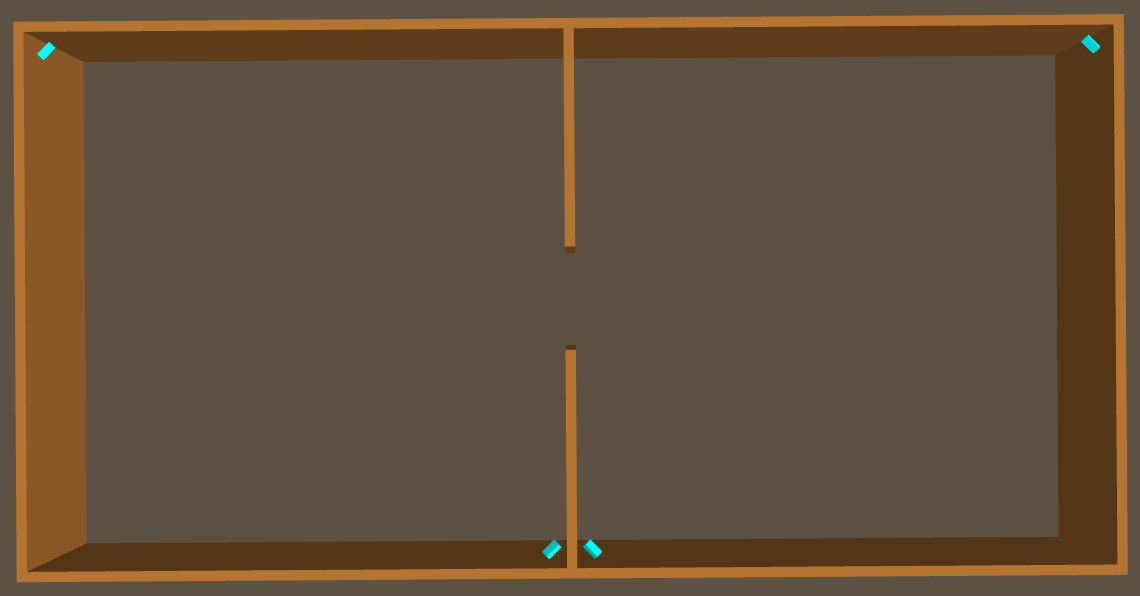
\includegraphics[width=\linewidth]{figures/two-room-horizontal.png}
            \caption{2-room horizontal layout.}
      \end{subfigure}
      \hfill
      \begin{subfigure}[t]{0.31\textwidth}
            \centering
            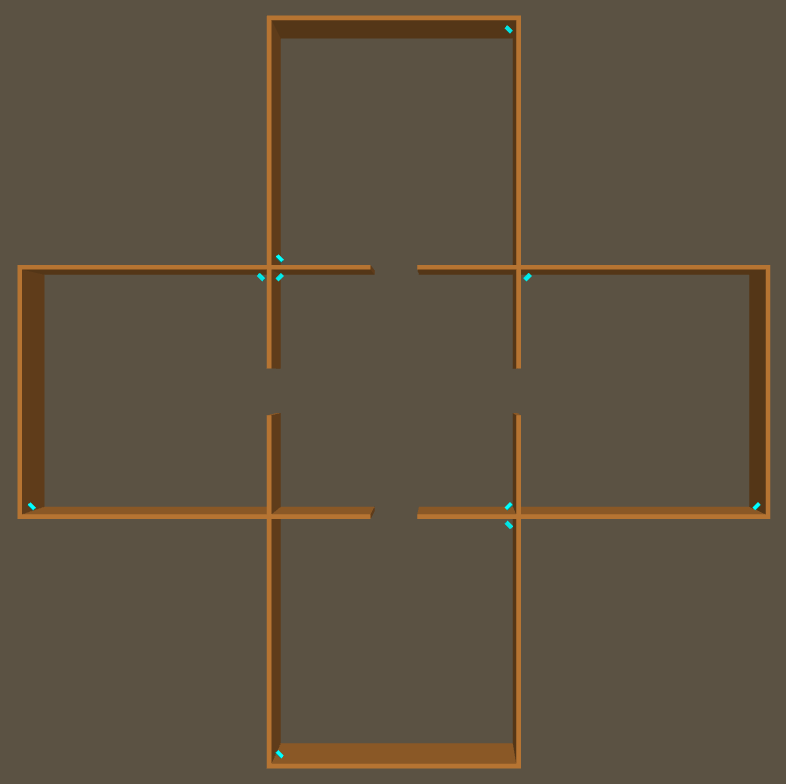
\includegraphics[width=\linewidth]{figures/five-room-star.png}
            \caption{5-room cross layout.}
      \end{subfigure}
      \hfill
      \begin{subfigure}[t]{0.31\textwidth}
            \centering
            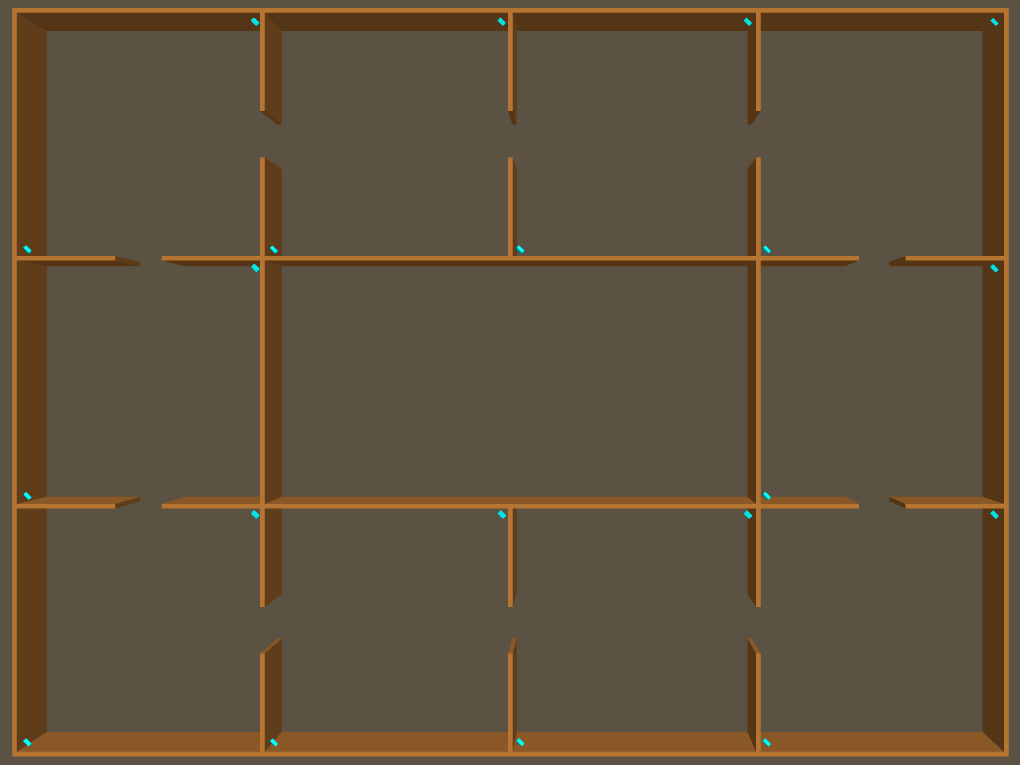
\includegraphics[width=\linewidth]{figures/ten-room-ring.png}
            \caption{10-room ring layout.}
      \end{subfigure}
      \caption{Top-down Gazebo layouts used in the evaluation for the 2-room,
                   5-room, and 10-room scenarios. Blue diamonds indicate the
                   fixed camera locations.}
      \label{fig:worlds}
\end{figure*}

\subsection{Robot Platform}

\begin{figure}[t]
    \centering
    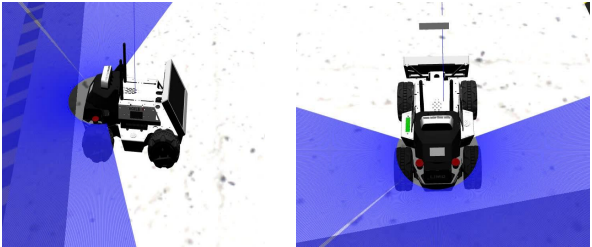
\includegraphics[width=\linewidth]{figures/robot_limo.png}
    \caption{The AgileX LIMO mobile robot used in simulation, shown from
             two viewpoints. The blue cone indicates the LiDAR field of view.}
    \label{fig:robot_limo}
\end{figure}

The simulated robot is an AgileX LIMO (Figure~\ref{fig:robot_limo}) with a 2D LiDAR
(range \SI{12}{\metre}, \SI{360}{\degree}, \SI{10}{\hertz}) and differential-drive
kinematics.
The robot is spawned at position $(x, y) = (4.0, 4.0)\ \si{\metre}$ in the
Gazebo world frame.

\subsection{SLAM Configuration}

We build on \emph{SLAM Toolbox}~\cite{macenski2021slamtoolbox}, the
de-facto standard 2D LiDAR SLAM framework in ROS~2.
SLAM Toolbox has been widely adopted across diverse mobile-robot
applications---from long-range autonomous navigation~\cite{macenski2021slam}
to multi-floor building mapping and warehouse logistics---making it a
representative and reproducible baseline for indoor SLAM research.
It is run in synchronous mapping mode with the following parameters:
map resolution \SI{0.05}{\metre/\text{cell}},
scan-match every \SI{0.5}{\second},
loop-closure minimum score $0.55$.
The Ceres solver~\cite{ceres-solver} uses SPARSE\_NORMAL\_CHOLESKY with a
Levenberg--Marquardt trust region.

\subsection{Baselines}

\begin{enumerate}
    \item \textbf{LiDAR-only SLAM}: the same SLAM backend with no camera
          constraints.
    \item \textbf{Camera-constrained SLAM} (ours): identical configuration
          with camera constraints enabled ($\sigma_x=\sigma_y=0.1$,
          $\sigma_\theta=0.05$).
\end{enumerate}

\subsection{Metrics}

We report:
\begin{itemize}
    \item \textbf{ATE} (Absolute Trajectory Error)~\cite{sturm2012benchmark}:
          RMSE between estimated and ground-truth poses over the full trajectory.
    \item \textbf{Map consistency}: overlap integral between the produced
          OccupancyGrid and the ground-truth map (intersection over union of
          occupied cells).
    \item \textbf{Camera marker error}: Euclidean distance from the orange
          (estimated) camera marker to the yellow (GT) camera marker in RViz,
          averaged across all cameras at the end of one lap.
\end{itemize}

Each condition was run $N=5$ times with randomised initial heading to assess
variance.
